\chapter{Governing equations}
{\bf \Large
\begin{tabular}{ccc}
\hline
  Correnspoinding author & : & Hirofumi Tomita\\
\hline
\end{tabular}
}

\section{Continuity equations}

The continuity equations for each material can be described as the flux form:
\begin{eqnarray}
&&  \frac{\partial \rho q_d}{\partial t}
+ \nabla \cdot\left(\rho q_d{\bf u}\right)  = {\rm DIFF}\left[q_d\right]
\label{eq:rho_d}\\
&&  \frac{\partial \rho q_v}{\partial t}
+ \nabla \cdot\left(\rho q_v {\bf u}\right)  = S_v + {\rm DIFF}\left[q_v\right]
\label{eq:rho_v}\\
&&  \frac{\partial \rho q_l}{\partial t}
+ \nabla \cdot\left(\rho q_l {\bf u}\right)
+ \frac{\partial \rho q_l w_l}{\partial z}=S_l + {\rm DIFF}\left[q_l\right]
\label{eq:rho_l}\\
&&  \frac{\partial \rho q_s}{\partial t}
+ \nabla \cdot\left(\rho q_s {\bf u}\right)
+ \frac{\partial \rho q_s w_s}{\partial z}=S_s + {\rm DIFF}\left[q_s\right]
\label{eq:rho_s}
\end{eqnarray}
The summation of the mass concentrations should be unit:
\begin{eqnarray}
&& q_d + q_v + q_l + q_s = 1. \label{eq:total_massconcentration}
\end{eqnarray}
The source terms of water substances should satisfy the following relation:
\begin{eqnarray}
  S_v + S_l + S_s = 0.
\end{eqnarray}
The summation of Eqs.(\ref{eq:rho_d})-(\ref{eq:rho_s}) gives the
continuity equation of total density:
\begin{eqnarray}
&&  \frac{\partial \rho}{\partial t}
+ \nabla\cdot\left(\rho{\bf u}\right)
+ \frac{\partial \rho q_l w_l}{\partial z}
+ \frac{\partial \rho q_s w_s}{\partial z}
=0, \label{eq:rhotot}
\end{eqnarray}
For this derivation,
we assume that
the operator ${ \rm DIFF}\left[\right]$ is distributive.
Using Eq.(\ref{eq:total_massconcentration}),
\begin{eqnarray}
&&  { \rm DIFF}\left[q_d\right]
+{ \rm DIFF}\left[q_v\right]
+{ \rm DIFF}\left[q_l\right]
+{ \rm DIFF}\left[q_s\right]\nonumber\\
&=&{ \rm DIFF}\left[q_d+q_v+q_l+q_s\right]
={ \rm DIFF}\left[1\right] = 0
\end{eqnarray}

\section{Momentum equations}

The momentum equations for the gas, liquid, and solid material
are described as
\begin{eqnarray}
&&  \frac{\partial \rho \left(q_d+q_v\right) {\bf u}}{\partial t}
+ \nabla \cdot \left[\rho \left(q_d+q_v\right){\bf u} \otimes {\bf u}\right]\\
&=&
-\nabla p - \left[\rho \left(q_d+q_v\right)g + (f_l+f_s)\right] {\bf e_z}\nonumber\\
&&+{\bf u} S_v +{\rm DIFF}\left[(q_d+q_v){\bf u}\right]
\label{eq:momgas}\\
&&  \frac{\partial \rho q_l {\bf u}}{\partial t}
+ \nabla \cdot \left(\rho q_l{\bf u} \otimes {\bf u}\right)
+ \frac{\partial \rho q_l {\bf u} w_l}{\partial z}
=
 - \left(\rho q_l g - f_l\right) {\bf e_z}\nonumber\\
&&+{\bf u} S_l+{\rm DIFF}\left[q_l{\bf u}\right]
\label{eq:momliquid}\\
&&  \frac{\partial \rho q_s {\bf u}}{\partial t}
+ \nabla \cdot \left(\rho q_s{\bf u} \otimes {\bf u}\right)
+ \frac{\partial \rho q_s {\bf u }w_s}{\partial z}
=
 - \left(\rho q_s g - f_s\right) {\bf e_z}\nonumber\\
&&+{\bf u} S_s+{\rm DIFF}\left[q_s{\bf u}\right]
\label{eq:momsolid}
\end{eqnarray}
The pressure is derived from the equation of state as
\begin{eqnarray}
p=\rho \left(q_d R_d + q_v R_v\right) T.\label{eq:state}
\end{eqnarray}
The summation of Eqs.(\ref{eq:momgas})-(\ref{eq:momsolid})
gives the total momentum equation as
\begin{eqnarray}
&&  \frac{\partial \rho {\bf u}}{\partial t}
+ \nabla \cdot \left(\rho{\bf u} \otimes {\bf u}\right)
+ \left(\frac{\partial \rho q_l w_l}{\partial z}
+ \frac{\partial \rho q_s w_s}{\partial z}\right) {\bf e_z}\nonumber\\
&=&
-\nabla p - \rho g {\bf e_z}
+{\rm DIFF}\left[{\bf u}\right]
\label{eq:momtot}
\end{eqnarray}
Note that the drag forces by water loading does not appear
in Eq.(\ref{eq:momtot}),
because those term are cancelled out through the summation.

\section{Thermodynamics equations}

The equations of the internal energies are described as
\begin{eqnarray}
&&  \frac{\partial \rho (q_d e_d + q_v e_v) }{\partial t} +
  \nabla \cdot \left[ \rho (q_d e_d + q_v e_v ){\bf u} \right] \nonumber\\
&=& - p \nabla \cdot {\bf u} + Q_{d}+ Q_{v} + {\rm DIFF}\left[(q_d+q_v)T^{*} \right]
\label{eq:thermogas}\\
&&  \frac{\partial \rho q_l e_l}{\partial t} +
  \nabla \cdot \left( \rho q_l e_l {\bf u} \right)
+ \frac{\partial \rho q_l e_l w_l}{\partial z}
= Q_l + {\rm DIFF}\left[q_l T^{*} \right]
\label{eq:thermoliquid}\\
&&  \frac{\partial \rho q_l e_s}{\partial t} +
  \nabla \cdot \left( \rho q_s e_s {\bf u} \right)
+ \frac{\partial \rho q_s e_s w_s}{\partial z}
= Q_s + {\rm DIFF}\left[q_s T^{*} \right]
\label{eq:thermosolid}
\end{eqnarray}
where $T^*$ is some kind of potential temperature, discussed later.
The internal energies are defined as
\begin{eqnarray}
&& e_d = c_{vd} T\\
&& e_v = c_{vv} T\\
&& e_l = c_{l} T\\
&& e_s = c_{s} T,
\end{eqnarray}
The summation of Eqs.(\ref{eq:thermogas})-(\ref{eq:thermosolid})
gives the following internal energy equations:
\begin{eqnarray}
&&  \frac{\partial \rho e  }{\partial t}
+  \nabla \cdot \left( \rho e {\bf u} \right)
+ \frac{\partial \rho q_l e_l w_l}{\partial z}
 + \frac{\partial \rho q_s e_s w_s}{\partial z}
 + p \nabla \cdot {\bf u}\nonumber\\
&=&  Q + {\rm DIFF}\left[T^{*} \right]
\label{eq:etot}
\end{eqnarray}
where
\begin{eqnarray}
&&  e = q_d e_d + q_v e_v + q_l e_l + q_s e_s,
\end{eqnarray}
and the total diabatic heating is described as
\begin{eqnarray}
&&  Q = Q_d + Q_v + Q_l + Q_s.
\end{eqnarray}

\section{Conseptual seperation for solving the set of equations}

Eqs.(\ref{eq:rho_v})-(\ref{eq:rho_s}),(\ref{eq:rhotot}),(\ref{eq:momtot}),
and (\ref{eq:state}) with Eq.(\ref{eq:etot}) are the complete set of equations.
For solving them easily, we seperate the set of equations conceptually as
\begin{eqnarray}
&&  \frac{\partial \phi}{\partial t} =
\left(\frac{\partial \phi}{\partial t}\right)_{dynamics}
+\left(\frac{\partial \phi}{\partial t}\right)_{physics}
\end{eqnarray}
The falling proccess of liquid and solid waters,
the source and sink process of water vapor, and
the diabatic heating process for energy equations are treated
as physical process, the others are treated as dynamical proccess.

According to this scheme,
the dynamical process can be written as
\begin{eqnarray}
&&  \frac{\partial \rho q_v}{\partial t}
+ \nabla \cdot\left(\rho q_v {\bf u}\right)  = 0
\label{eq:rho_v_d}\\
&&  \frac{\partial \rho q_l}{\partial t}
+ \nabla \cdot\left(\rho q_l {\bf u}\right) = 0
\label{eq:rho_l_d}\\
&&  \frac{\partial \rho q_s}{\partial t}
+ \nabla \cdot\left(\rho q_s {\bf u}\right)
= 0
\label{eq:rho_s_d}\\
&&  \frac{\partial \rho}{\partial t}
+ \nabla\cdot\left(\rho{\bf u}\right)
=0 \label{eq:rhotot_d}\\
&&  \frac{\partial \rho {\bf u}}{\partial t}
+ \nabla \cdot \left(\rho{\bf u} \otimes {\bf u}\right)
=
-\nabla p - \rho g {\bf e_z} \label{eq:momtot_d}\\
&&  \frac{\partial \rho e  }{\partial t}
+  \nabla \cdot \left( \rho e {\bf u} \right)
 + p \nabla \cdot {\bf u}
=  0 \label{eq:etot_d}
\end{eqnarray}

On the other hand,
the physical processes are as follows:
\begin{eqnarray}
&&  \frac{\partial \rho q_v}{\partial t}  = S_v
+{\rm DIFF}\left[q_v \right]
\label{eq:rho_v_p}\\
&&  \frac{\partial \rho q_l}{\partial t}
+ \frac{\partial \rho q_l w_l}{\partial z}=S_l
+{\rm DIFF}\left[q_l \right]
\label{eq:rho_l_p}\\
&&  \frac{\partial \rho q_s}{\partial t}
+ \frac{\partial \rho q_s w_s}{\partial z}=S_s
+{\rm DIFF}\left[q_s \right]
\label{eq:rho_s_p}\\
&&  \frac{\partial \rho}{\partial t}
+ \frac{\partial \rho q_l w_l}{\partial z}
+ \frac{\partial \rho q_s w_s}{\partial z}
=0 \label{eq:rhotot_p}\\
&&  \frac{\partial \rho {\bf u}}{\partial t}
+ \frac{\partial \rho q_l {\bf u} w_l}{\partial z}
+ \frac{\partial \rho q_s {\bf u} w_s}{\partial z}
= {\rm DIFF}\left[{\bf u} \right]
 \label{eq:momtot_p}\\
&&  \frac{\partial \rho e  }{\partial t}
+ \frac{\partial \rho q_l e_l w_l}{\partial z}
 + \frac{\partial \rho q_s e_s w_s}{\partial z}
=  Q + {\rm DIFF}\left[T^{*} \right] \label{eq:etot_p}
\end{eqnarray}

\section{Conservation of thermodynamics in the dynamical process}

Equation (\ref{eq:etot_d}) is not a complete flux form,
because the internal energy itself is not conserved
both in the Euler sense and in the Lagrangian sense.
In this section, we consider the conservative
quantity for thermodynamics equation.

In the dry atmosphere, the potential temperature for dry air,
which is defined as
\begin{eqnarray}
\theta_d &=& T \left(\frac{p_{00}}{p}\right)^{R_d/c_{pd}},
\end{eqnarray}
is used as a conserved quantity it is conserved along the Lagrange trajectory
$c_{pd}$ $R_d$ are the specific heats at constant pressure and
However, it is no longer satisfied when the water substances are included.

Sinece Eq.(\ref{eq:rhotot_d}) is equivallent to
\begin{eqnarray}
  \frac{d \rho}{dt}+\rho \nabla \cdot {\bf u} = 0,
\end{eqnarray}
Equation (\ref{eq:etot_d}) is
\begin{eqnarray}
  \rho \frac{de}{dt} - \frac{p}{\rho}\frac{d \rho}{dt} =0. \label{eq:etot_d2}
\end{eqnarray}
Dividing by $\rho$, this equation can be written as
\begin{eqnarray}
  \frac{de}{dt} + p \frac{d}{dt}\left(\frac{1}{\rho}\right) = 0.
\label{eq:thermodyn}
\end{eqnarray}
Substiting Eq.(\ref{eq:state}) into Eq.(\ref{eq:thermodyn}),
\begin{eqnarray}
&& \frac{d  q_d c_{vd}   T}{dt} + p \frac{d}{dt} \left[\frac{q_d R_d T}{p}\right]
+\frac{d  q_v c_{vv}   T}{dt} + p \frac{d}{dt} \left[\frac{q_v R_v T}{p}\right]
\nonumber\\
&&+\frac{d  q_l c_{l}   T}{dt}+\frac{d  q_s c_{s}   T}{dt} =0
\label{eq:thermodyn_dash}
\end{eqnarray}

Since Eqs.(\ref{eq:rho_v_d})-(\ref{eq:rhotot_d}) give
\begin{eqnarray}
  \frac{d q_d}{dt} = \frac{d q_v}{dt} = \frac{d q_l}{dt} = \frac{d q_s}{dt} = 0,
\end{eqnarray}
Equation (\ref{eq:thermodyn_dash}) gives the following form:
\begin{eqnarray}
&& q_d  \left[\frac{d  c_{vd}   T}{dt} +  p \frac{d}{dt} \left[\frac{ R_d T}{p}\right]\right]
+q_v \left[\frac{d  c_{vv}   T}{dt} + p \frac{d}{dt} \left[\frac{ R_v T}{p}\right]\right]\nonumber\\
&&+ q_l  \frac{d  c_{l}   T}{dt} + q_s  \frac{d  c_{s}   T}{dt} =0
\end{eqnarray}
Dividing this equation by $T$,
\begin{eqnarray}
%1
&&q_d  \left[c_{pd} \frac{1}{T}\frac{d T}{dt}
+  R_d p \frac{d}{dt} \left(\frac{1}{p}\right)\right]
+q_v  \left[c_{pv} \frac{1}{T}\frac{d T}{dt}
+  R_v p \frac{d}{dt} \left(\frac{1}{p}\right)\right]\nonumber\\
&&+ q_l c_{l} \frac{1}{T}  \frac{d   T}{dt}
  + q_s c_{s} \frac{1}{T}  \frac{d   T}{dt} =0\\
%2
&&q_d c_{pd} \left[ \frac{d \ln T}{dt}
+  \frac{R_d}{c_{pd}} \frac{d}{dt} \left[\ln \left(\frac{1}{p}\right)\right]\right]
+q_v c_{pv}  \left[\frac{d \ln T}{dt}
+  \frac{R_v}{c_{pv}} \frac{d}{dt} \left[\ln \left(\frac{1}{p}\right)\right]\right]\nonumber\\
&&+ q_l c_{l}  \frac{d \ln T}{dt}
  + q_s c_{s}  \frac{d \ln T}{dt} =0 \label{eq:thermdyn2}\\
&&
 q_d c_{pd} \frac{d \ln \theta_d}{dt}
+q_v c_{pv} \frac{d \ln \theta_v}{dt}
+q_l c_l   \frac{d \ln T}{dt}
+q_s c_s   \frac{d  \ln T}{dt}=0\\
&&
\frac{d}{dt}\left[ \ln \left(
\theta_d^{q_d c_{pd}} \theta_v^{q_v c_{pv}} T^{q_l c_l} T^{q_s c_s}
\right)\right] = 0 \label{eq:lnThetaconserveation}
\end{eqnarray}
Thus,
\begin{eqnarray}
&&\frac{d}{dt}\left[
\theta_d^{q_d c_{pd}} \theta_v^{q_v c_{pv}} T^{q_l c_l} T^{q_s c_s}
\right] = 0
\end{eqnarray}
Thus, the following quantity is conserved along the flow trajectory;
\begin{eqnarray}
\Theta = \theta_d^{q_d c_{pd}} \theta_v^{q_v c_{pv}} T^{q_l c_l} T^{q_s c_s}
\end{eqnarray}
where $\theta_v$ is the potential temperature for water vapor, defined as
\begin{eqnarray}
\theta_v &=& T \left(\frac{p_{00}}{p}\right)^{R_v/c_{pv}}
\end{eqnarray}

The equation of state has the following expression using $\Theta$.
\begin{eqnarray}
\Theta &=&
T^{q_d c_{pd}} \left(\frac{p_{00}}{p}\right)^{q_d R_d}
T^{q_v c_{pv}} \left(\frac{p_{00}}{p}\right)^{q_v R_v}
T^{q_l c_l}  + T^{q_s c_s} \\
&=&
T^{q_d c_{pd} +q_vc_{pv}+q_lc_l+q_sc_s}
\left(\frac{p_{00}}{p}\right)^{q_d R_d + q_v R_v} \\
&=&
T^{c_p^*}\left(\frac{p_{00}}{p}\right)^{R^*},
\end{eqnarray}
where
\begin{eqnarray}
  c_p^* &\equiv& q_d c_{pd} +q_vc_{pv}+q_lc_l+q_sc_s\\
  R^* &\equiv& q_d R_d + q_v R_v
\end{eqnarray}
We define a new potential temperature
\begin{eqnarray}
\theta \equiv \Theta^{1/c_p^*} &=& T \left(\frac{p_{00}}{p}\right)^{R^*/c_p^*}
%&=& T \left(\frac{p_{00}}{p}\right)^{\frac{R_d}{c_{pd}} \alpha}
\end{eqnarray}
%% where
%% \begin{eqnarray}
%%   \alpha &=& \frac{q_d + q_v \frac{R_v}{R_d}}{q_d + q_v \frac{c_{pv}}{c_{pd}}+q_l\frac{c_l}{c_{pd}}
%% +q_s\frac{c_s}{c_{pd}}}
%% \end{eqnarray}

The pressure expression is derived diagnostically as follows:
\begin{eqnarray}
p&=&\rho (q_d R_d + q_v R_v) \theta \left(\frac{p}{p_{00}}\right)^{\frac{R^*}{c_{p}^*}}\\
p^{1-\frac{R^*}{c_{p}^*}}&=&\rho R^* \theta \left(\frac{1}{p_{00}}\right)^{\frac{R^*}{c_{p}^*}}\\
p&=&p_{00}\left(\frac{\rho \theta R^*}{p_{00}} \right)^{\frac{c_{p}^*}{c_{p}^*- R^*}} \label{eq: pressure}
\end{eqnarray}

Note that
\begin{eqnarray}
  \frac{d \theta}{dt} = \frac{1}{a} \Theta^{1/a-1} \frac{d \Theta}{dt} = 0
  \label{eq:theta_theta_relation}
\end{eqnarray}
Therefore, $\rho \theta$ can be employed for the prognostic varaiable!

Figure \ref{fig:fig1}(a) gives the vertical profile of the temperature
in the U.S.standard atmosphere and Fig.\ref{fig:fig1}(b) shows
the vetical profiles of $\theta/\theta_d$ under this temperature condition
when we assume that $q_v$ is mass concentration of water vapor at the saturation,
$q_l+q_s$ gives 0.0, 0.01, 0.02, and 0.04.
The differnce between $\theta$ and $\theta_d$ becomes
larger with the height and it may not be negligible.

\section{Diabatic heating in the physical process}

If the prognostic variable for thermodynamics is changed
from the internal energy to the newly defined potential temperature $\theta$,
the diabatic heating in Eq.(\ref{eq:etot_p}) should be modified.
Through
the manupulation from Eq.(\ref{eq:etot_d2}) to Eq.(\ref{eq:lnThetaconserveation}),
Eq.(\ref{eq:etot_p}) without turbulence term can be written as
\begin{eqnarray}
  \frac{d \ln \Theta}{dt} = \frac{Q}{\rho T}
  \label{eq:dlntheta_dt}
\end{eqnarray}
On the other hand, Eq.(\ref{eq:theta_theta_relation}) gives
\begin{eqnarray}
  \frac{d \theta}{dt} = \frac{1}{c_p^*} \Theta^{1/a} \frac{d \ln \Theta}{dt}
  \label{eq:dtheta_dt}
\end{eqnarray}
Substituting Eq.(\ref{eq:dlntheta_dt}) into Eq.(\ref{eq:dtheta_dt}),
\begin{eqnarray}
  \frac{d \theta}{dt} = \frac{1}{c_p^*}
  \left(\frac{p}{p_{00}}\right)^{\frac{R^*}{c_p^*}} \frac{Q}{\rho}
\end{eqnarray}

\section{Summary of equations in the dynamical process and physical process}
\subsection{The dynamical process}
\begin{eqnarray}
&&  \frac{\partial \rho q_v}{\partial t}
+ \nabla \cdot\left(\rho q_v {\bf u}\right) = \left(\frac{\partial \rho q_v}{\partial t}\right)_{physics}
\label{eq:rho_v_d2}\\
&&  \frac{\partial \rho q_l}{\partial t}
+ \nabla \cdot\left(\rho q_l {\bf u}\right) = \left(\frac{\partial \rho q_l}{\partial t}\right)_{physics}
\label{eq:rho_l_d2}\\
&&  \frac{\partial \rho q_s}{\partial t}
+ \nabla \cdot\left(\rho q_s {\bf u}\right)
= \left(\frac{\partial \rho q_s}{\partial t}\right)_{physics}
\label{eq:rho_s_d2}\\
&&  \frac{\partial \rho}{\partial t}
+ \nabla\cdot\left(\rho{\bf u}\right)
= \left(\frac{\partial \rho}{\partial t}\right)_{physics}
 \label{eq:rhotot_d2}\\
&&  \frac{\partial \rho {\bf u}}{\partial t}
+ \nabla \cdot \left(\rho{\bf u} \otimes {\bf u}\right)
=
-\nabla p - \rho g {\bf e_z}
+\left(\frac{\partial \rho {\bf u}}{\partial t}\right)_{physics}
 \label{eq:momtot_d2}\\
&&  \frac{\partial \rho \theta  }{\partial t}
+  \nabla \cdot \left( \rho \theta {\bf u} \right) =
\left(\frac{\partial \rho \theta}{\partial t}\right)_{physics} \\
&& p=p_{00}\left(\frac{\rho \theta R^*}{p_{00}} \right)^{\frac{c_{p}^*}{c_{p}^*- R^*}}
\end{eqnarray}
where
\begin{eqnarray}
  c_p^* &\equiv& q_d c_{pd} +q_vc_{pv}+q_lc_l+q_sc_s\\
  R^* &\equiv& q_d R_d + q_v R_v
\end{eqnarray}

\subsection{The physical process}
\begin{eqnarray}
&& \left( \frac{\partial \rho q_v}{\partial t} \right)_{physics}  = S_v
+{\rm DIFF}\left[q_v \right]
\label{eq:rho_v_p2}\\
&& \left( \frac{\partial \rho q_l}{\partial t} \right)_{physics}
= - \frac{\partial \rho q_l w_l}{\partial z}+S_l
+{\rm DIFF}\left[q_l \right]
\label{eq:rho_l_p2}\\
&& \left( \frac{\partial \rho q_s}{\partial t} \right)_{physics}
=- \frac{\partial \rho q_s w_s}{\partial z}+S_s
+{\rm DIFF}\left[q_s \right]
\label{eq:rho_s_p2}\\
&& \left( \frac{\partial \rho}{\partial t} \right)_{physics}
=- \frac{\partial \rho q_l w_l}{\partial z}
 - \frac{\partial \rho q_s w_s}{\partial z}
 \label{eq:rhotot_p2}\\
&& \left( \frac{\partial \rho {\bf u}}{\partial t} \right)_{physics}
=
- \frac{\partial \rho q_l {\bf u} w_l}{\partial z}
- \frac{\partial \rho q_s {\bf u} w_s}{\partial z}
+{\rm DIFF}\left[{\bf u} \right]
 \label{eq:momtot_p2}\\
&& \left( \frac{\partial \rho \theta  }{\partial t} \right)_{physics}
=  \frac{1}{c_p^*} \left(\frac{p}{p_{00}}\right)^{\frac{R^*}{c_p^*}}
\left[Q
 - \frac{\partial \rho q_l e_l w_l}{\partial z}
 - \frac{\partial \rho q_s e_s w_s}{\partial z}
\right]
 + {\rm DIFF}\left[\theta \right] \label{eq:etot_p2}
\end{eqnarray}

\begin{figure}[t]
  (a)\\
  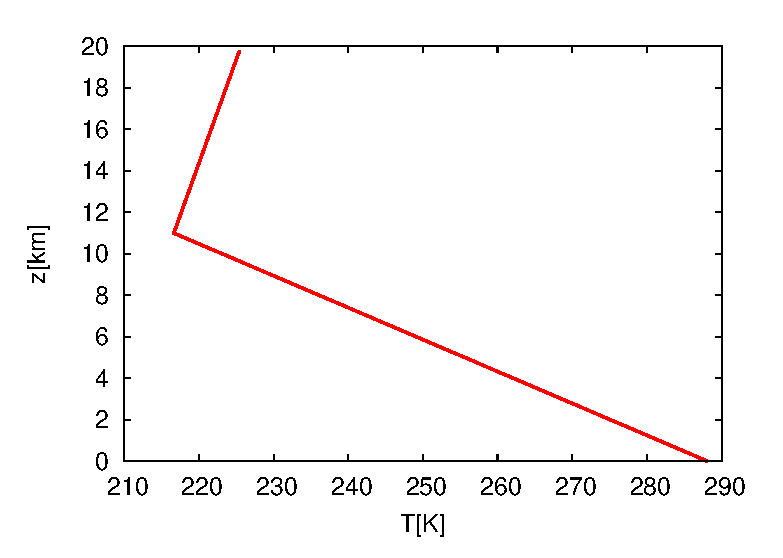
\includegraphics{./figure/us_std_atm_profile.eps}\\
  (b)\\
  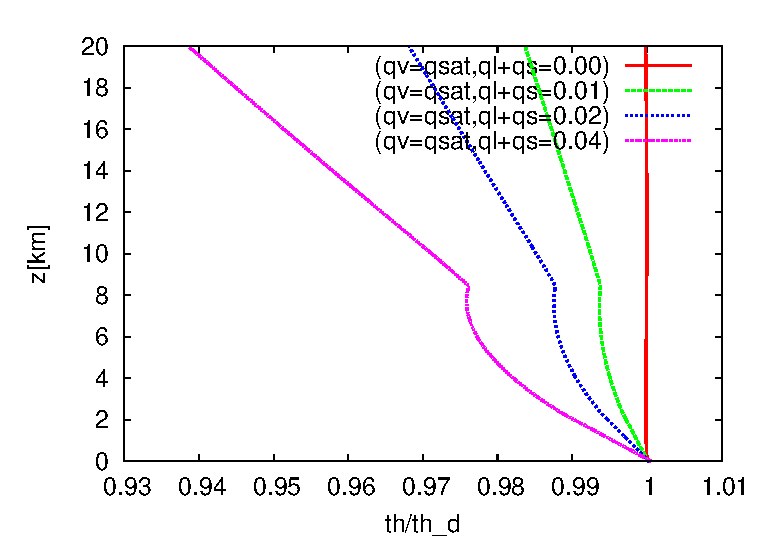
\includegraphics{./figure/theta_theta_d_profile.eps}\\
  \caption{Thee vertical profile of (a) U.S. standard atmosphere,
  (b) Several profiles of $\theta/\theta_d$.}
  \label{fig:fig1}
\end{figure}
